%%%%%%%%%%%%%%%%%%%%%%%%%%%%%%%%%%%%%%%%%%%%%%%%%%%%%%%%%%%%
%% introduction.tex
%%
%% Kapitel: Introduction
%% Autor: Axel Vierling (axel.vierling@cs.rptu.de)       
%% Autor: Jochen Hirth (j_hirth@informatik.uni-kl.de)       
%% Autor: Tobias Luksch (luksch@informatik.uni-kl.de)       
%% Datum: Juli 2003                                         
%%                                                          
%% Letzte Änderung Dezember 2023
%%%%%%%%%%%%%%%%%%%%%%%%%%%%%%%%%%%%%%%%%%%%%%%%%%%%%%%%%%%%
\chapter{Tables, Images, and More}
\label{chap:floats}
To ensure consistency in the appearance, labeling, and referencing of images, tables, etc., this chapter describes how these elements should be created.

%%%%%%%%%%%%%%%%%%%%%%%%%%%%%%%%%%%%%%%%%%%%%%%%%%%%%%%%%%%%
\section{Images}
\label{sec:floats:images}
\index{Images} Generally, it's advisable to create a dedicated directory for images, especially in larger documents, possibly categorizing them into folders for photos, drawings, plots, etc. These directories can be specified in the main file (refer to Chapter ~\ref{sec:class:main}). Since we're creating our document with \texttt{pdflatex}, images can be in pdf, jpeg, or png formats. For jpeg or png formats, it's crucial to ensure a sufficiently high resolution. If the illustrations are vector graphics in pdf format, ensure that all used fonts are embedded. For creating vector graphics (both in Windows and Linux), tools like \texttt{inkscape} are suitable. For image conversion, command-line tools like \texttt{mogrify} or \texttt{convert} are available in Linux. Additionally, a graphical tool like \texttt{gimp} can be used. 


To include images, something along the lines of:
\begin{verbatim}
   \begin{figure}
     \begin{center}
       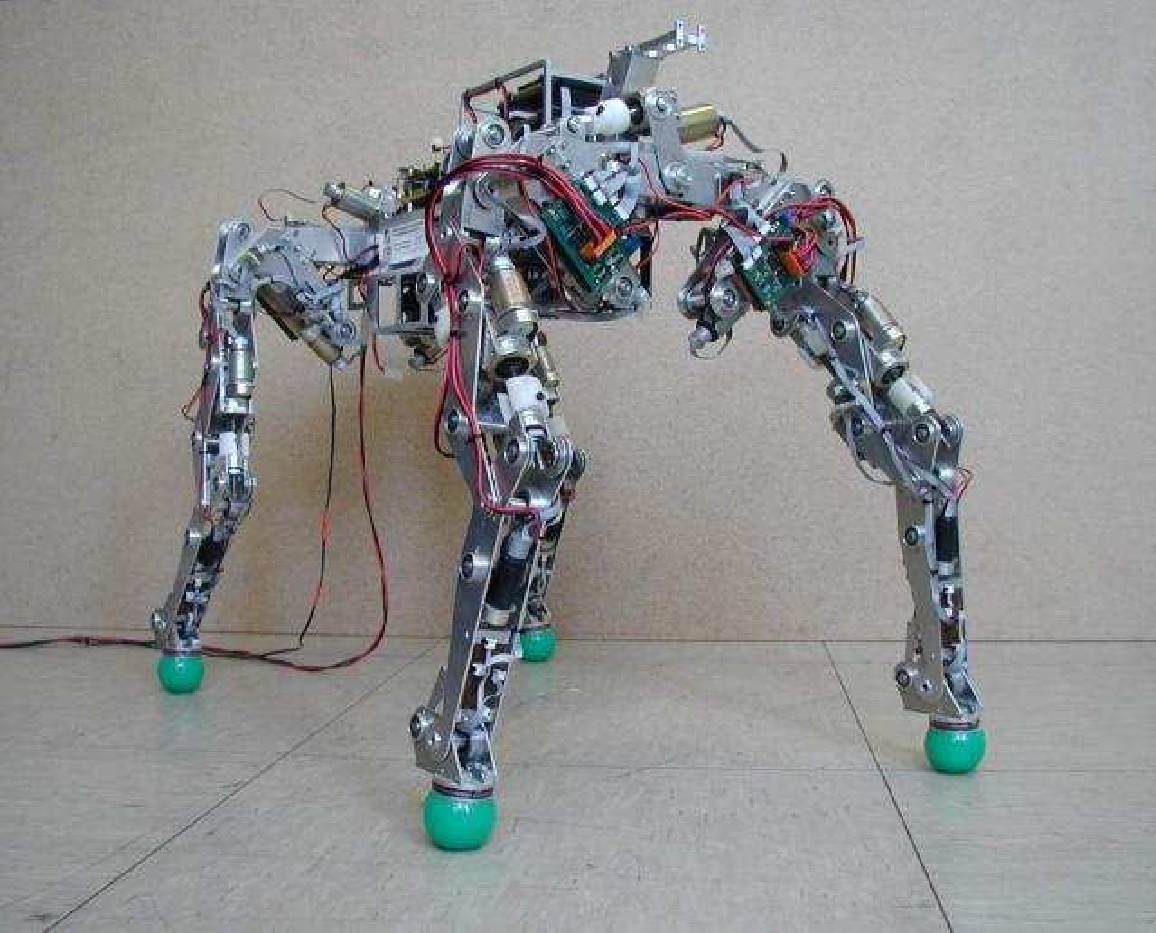
\includegraphics[width=5cm]{bisam}
       \caption{The quadrupedal walking machine Bisam developed at the Research Center
       for Information Technology in Karlsruhe.}
       \label{fig:bisam}
     \end{center}
   \end{figure}
\end{verbatim}
is used. This generates the output seen in~\ref{fig:bisam}.

\begin{figure}
  \begin{center}
    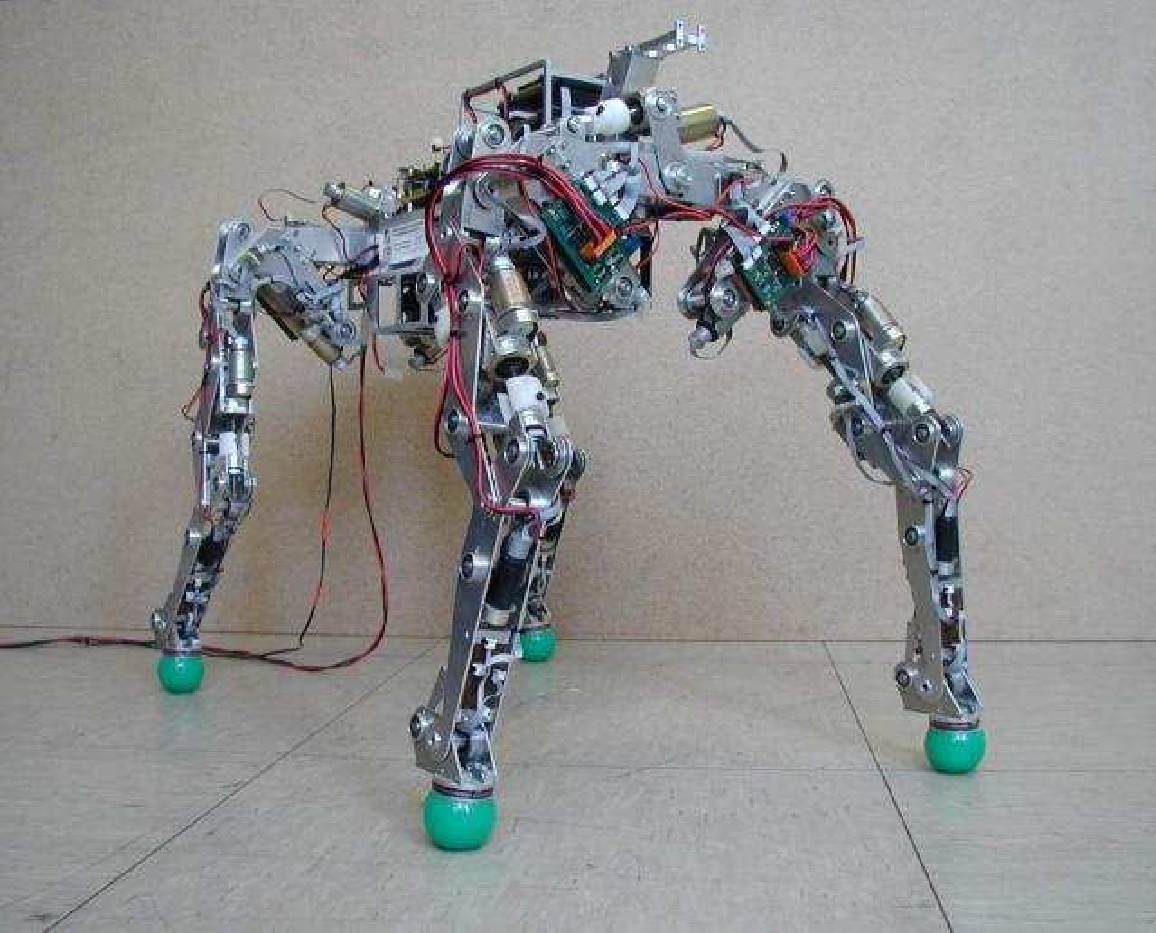
\includegraphics[width=5cm]{bisam}
    \caption{The quadrupedal walking machine Bisam developed at the Research Center
    for Information Technology in Karlsruhe.}
    \label{fig:bisam}
  \end{center}
\end{figure}

Specific commands and their parameters are referenced in appropriate literature. It's crucial that the image caption accurately describes what the image depicts. However, discussions about what's shown should be within the main text. For instance, if the figure is a plot, the caption might read: "Temperature trend with closed Valve B. Here, the temperature exceeds the critical limit at $t=\unit[130]{sec}$." The explanation of why this occurs, what effects are at play, or whether it's good or bad should not be under the image but discussed in the text. For data plots, ensure that all axes are properly labeled, and the legend is complete.

\begin{figure}
  \begin{subfigure}[b]{.5\linewidth}
    \centering 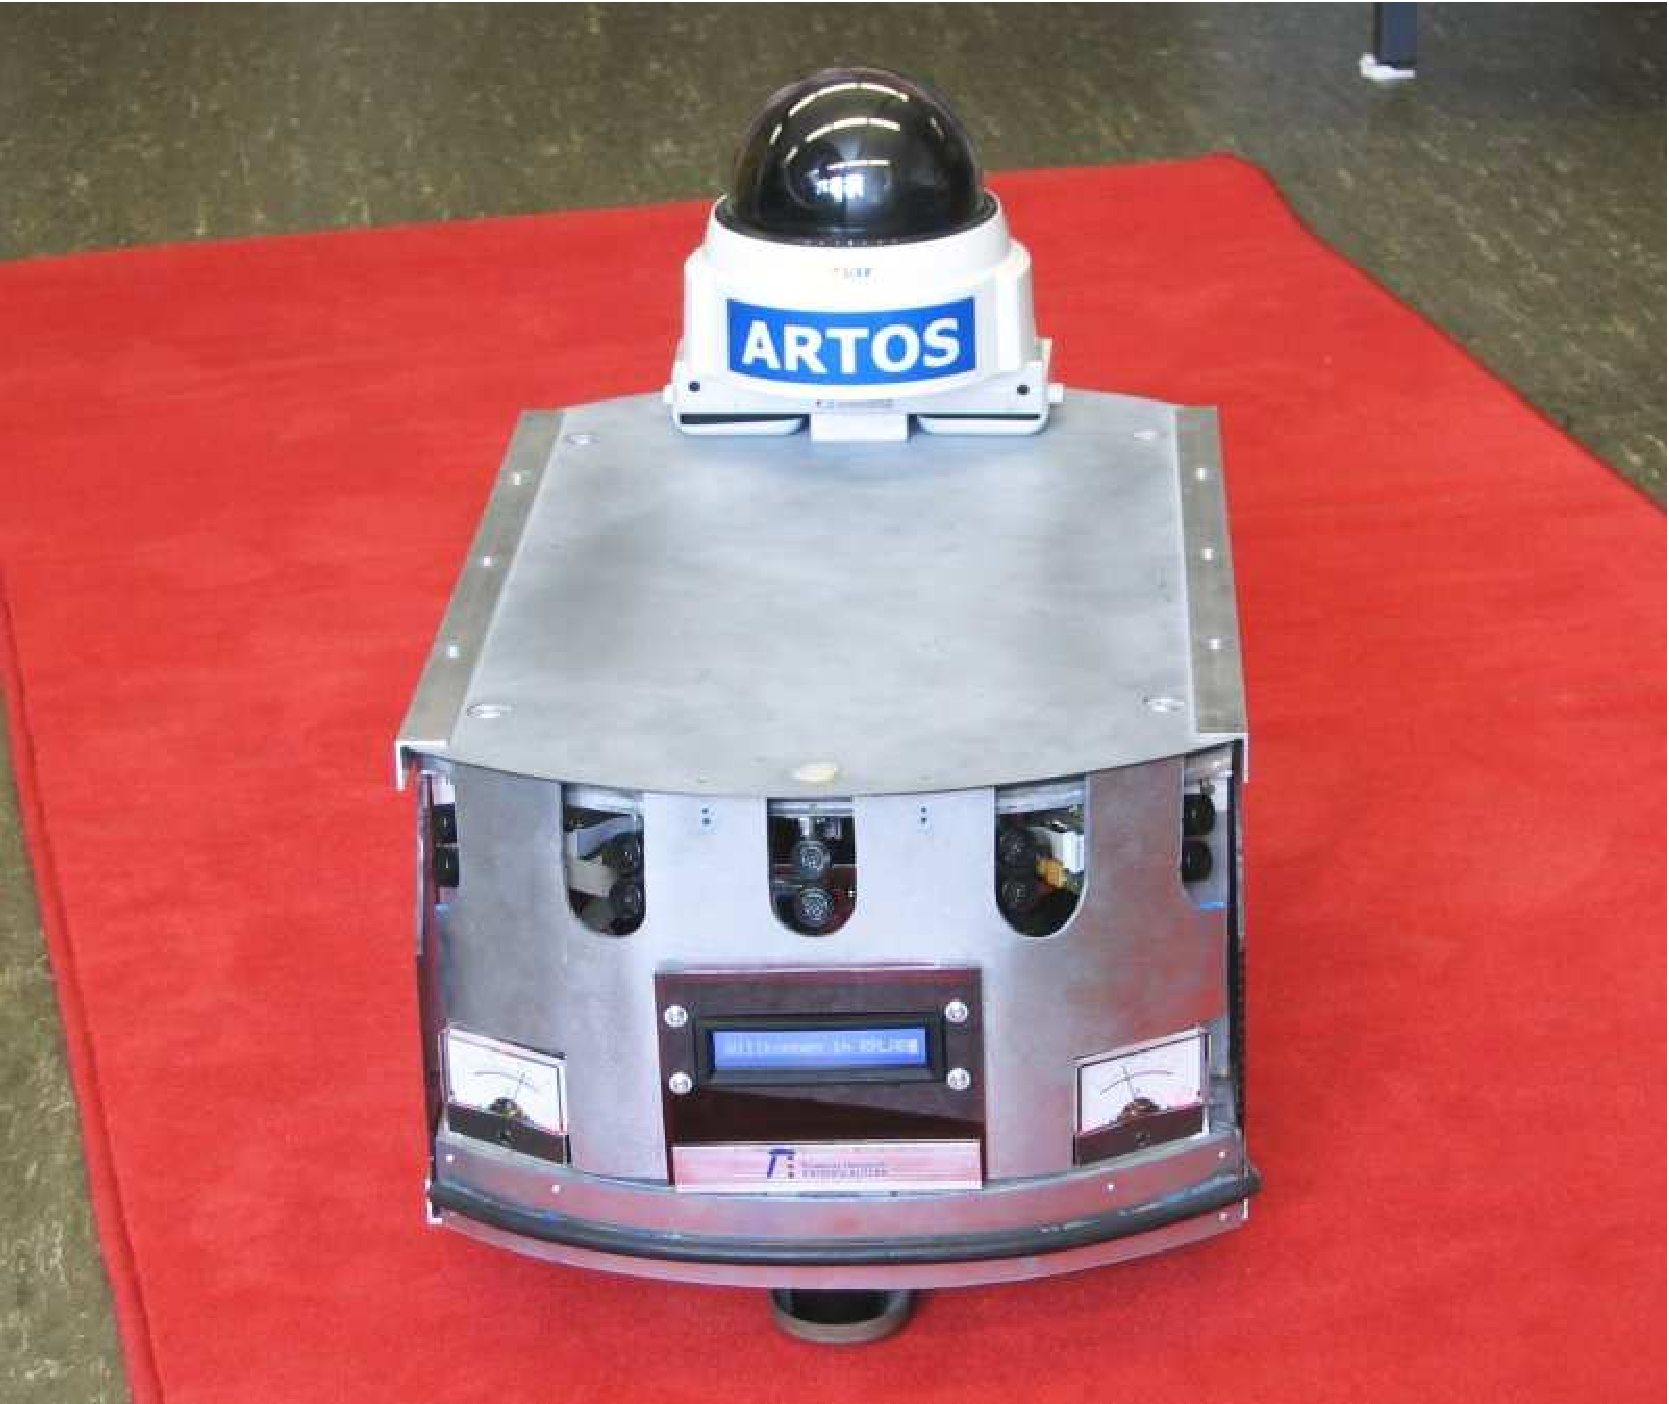
\includegraphics[height=5cm]{images/roter_teppich}
    \caption{\RRLABartos}
    \label{subfig:artos}
  \end{subfigure}%
  \hspace{1cm}
  \begin{subfigure}[b]{.5\linewidth}
    \centering 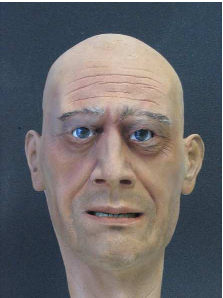
\includegraphics[height=5cm]{images/roman_mask}
    \caption{\RRLABroman}
    \label{subfig:roman}
  \end{subfigure}
  \caption{The mobile robot artos \RRLABartos (Autonomous Robot for Transport and Service)
  \subref{subfig:artos}  and the humanoid robot \RRLABroman (RObot huMAN interaction machine)
  \subref{subfig:roman}.}
  \label{fig:artos_and_roman}
\end{figure}

To include multiple images within a float environment, use something similar to:
\begin{verbatim}
\begin{figure}
  \begin{subfigure}[b]{.5\linewidth}
    \centering 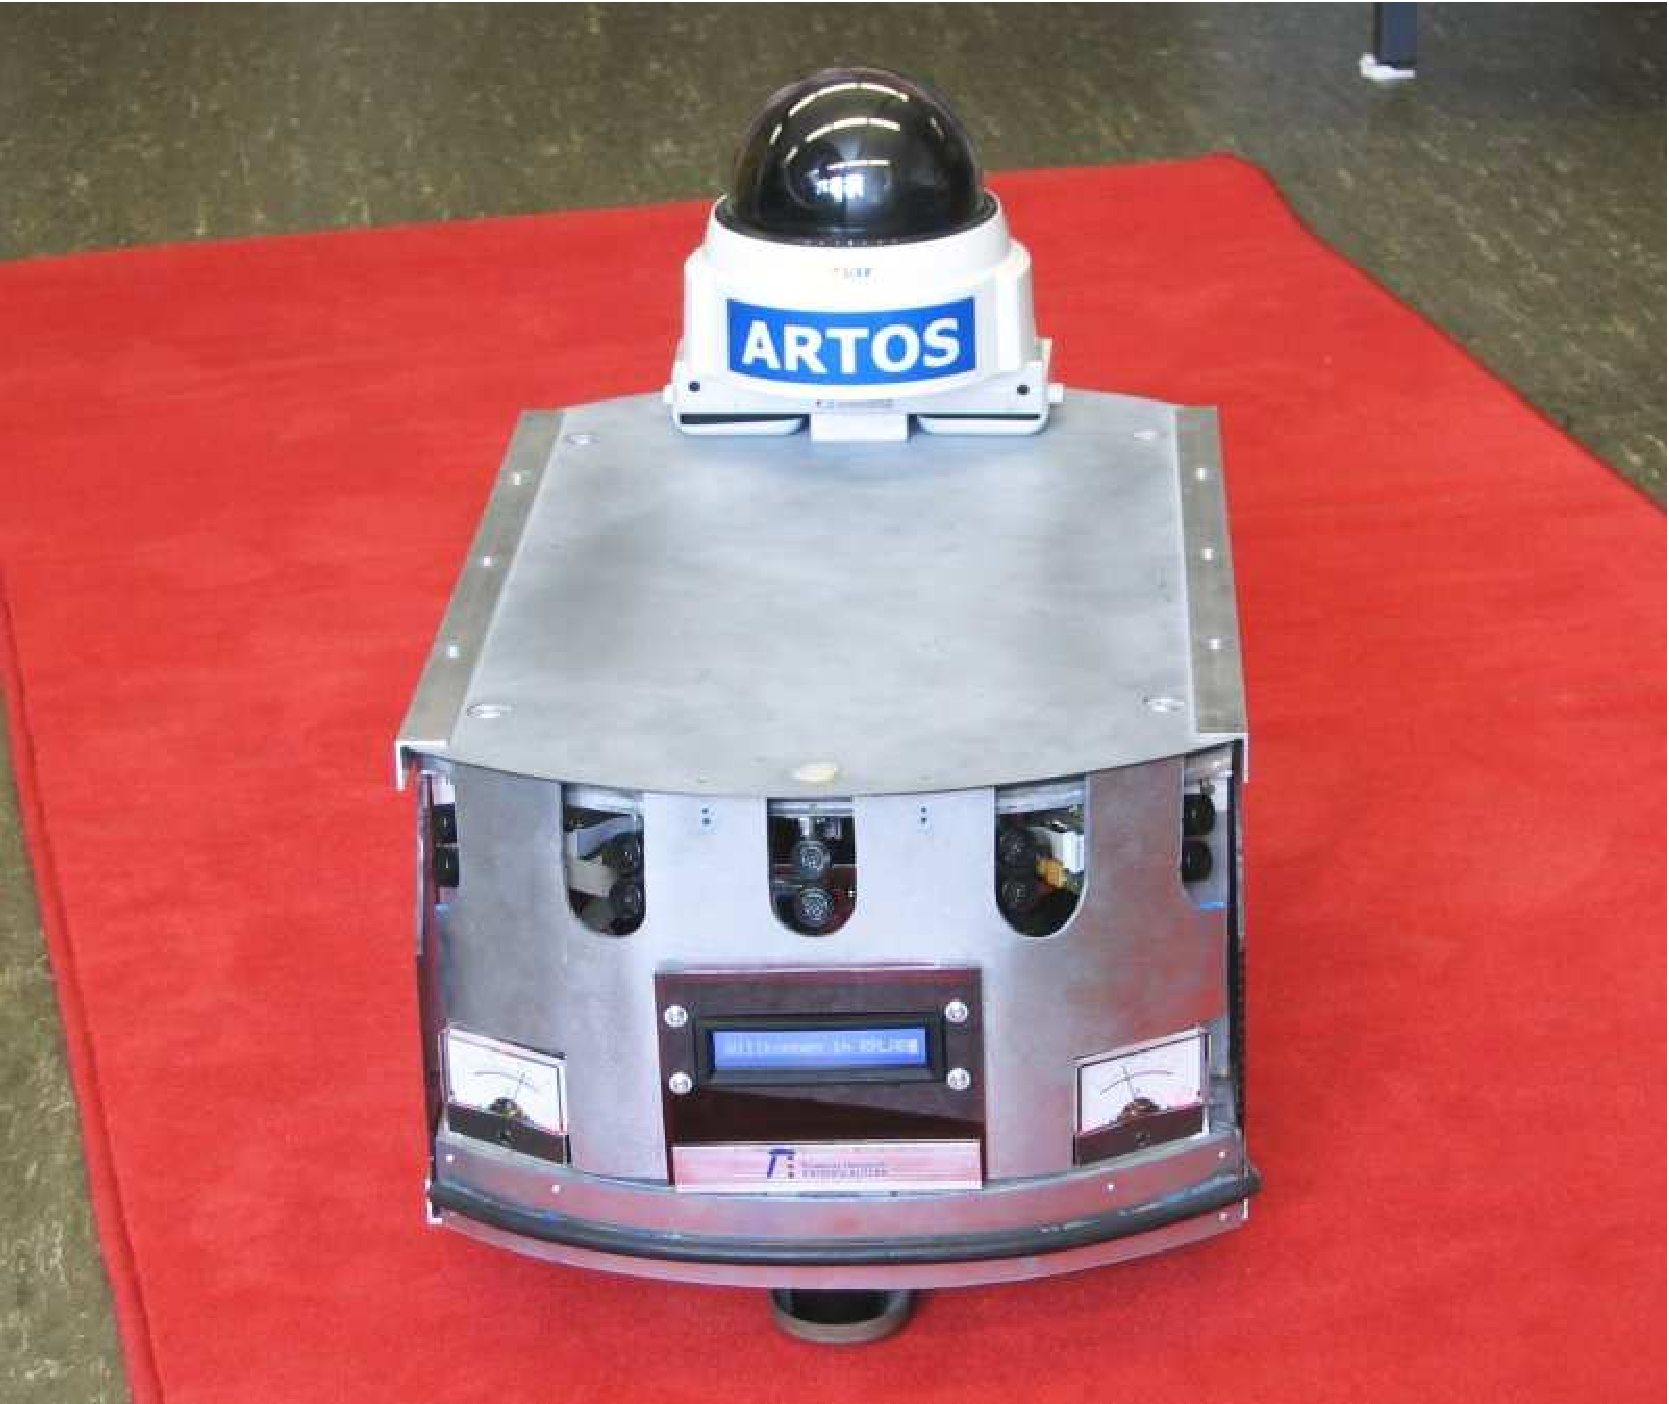
\includegraphics[height=5cm]{images/roter_teppich}
    \caption{\RRLABartos}
    \label{subfig:artos}
  \end{subfigure}%
  \hspace{1cm}
  \begin{subfigure}[b]{.5\linewidth}
    \centering 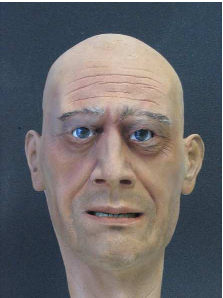
\includegraphics[height=5cm]{images/roman_mask}
    \caption{\RRLABroman}
    \label{subfig:roman}
  \end{subfigure}
  \caption{The mobile robot artos \RRLABartos (Autonomous Robot for Transport and Service)
  \subref{subfig:artos}  and the humanoid robot \RRLABroman (RObot huMAN interaction machine)
  \subref{subfig:roman}.}
  \label{fig:artos_and_roman}
\end{figure}
\end{verbatim}

This generates the output seen in Figure~\ref{fig:artos_and_roman}.

Alternatively, a ,,minipage'' can be used, as in Figures~\ref{fig:ARTOS} and~\ref{fig:ROMAN}. The ,,subfig'' variant is suitable when images are closely related and meant to be referenced as a single figure. The "minipage" is practical when both images are referenced separately.

\begin{figure}
  \begin{center}
    \begin{minipage}{0.48\textwidth}
      \begin{center}
        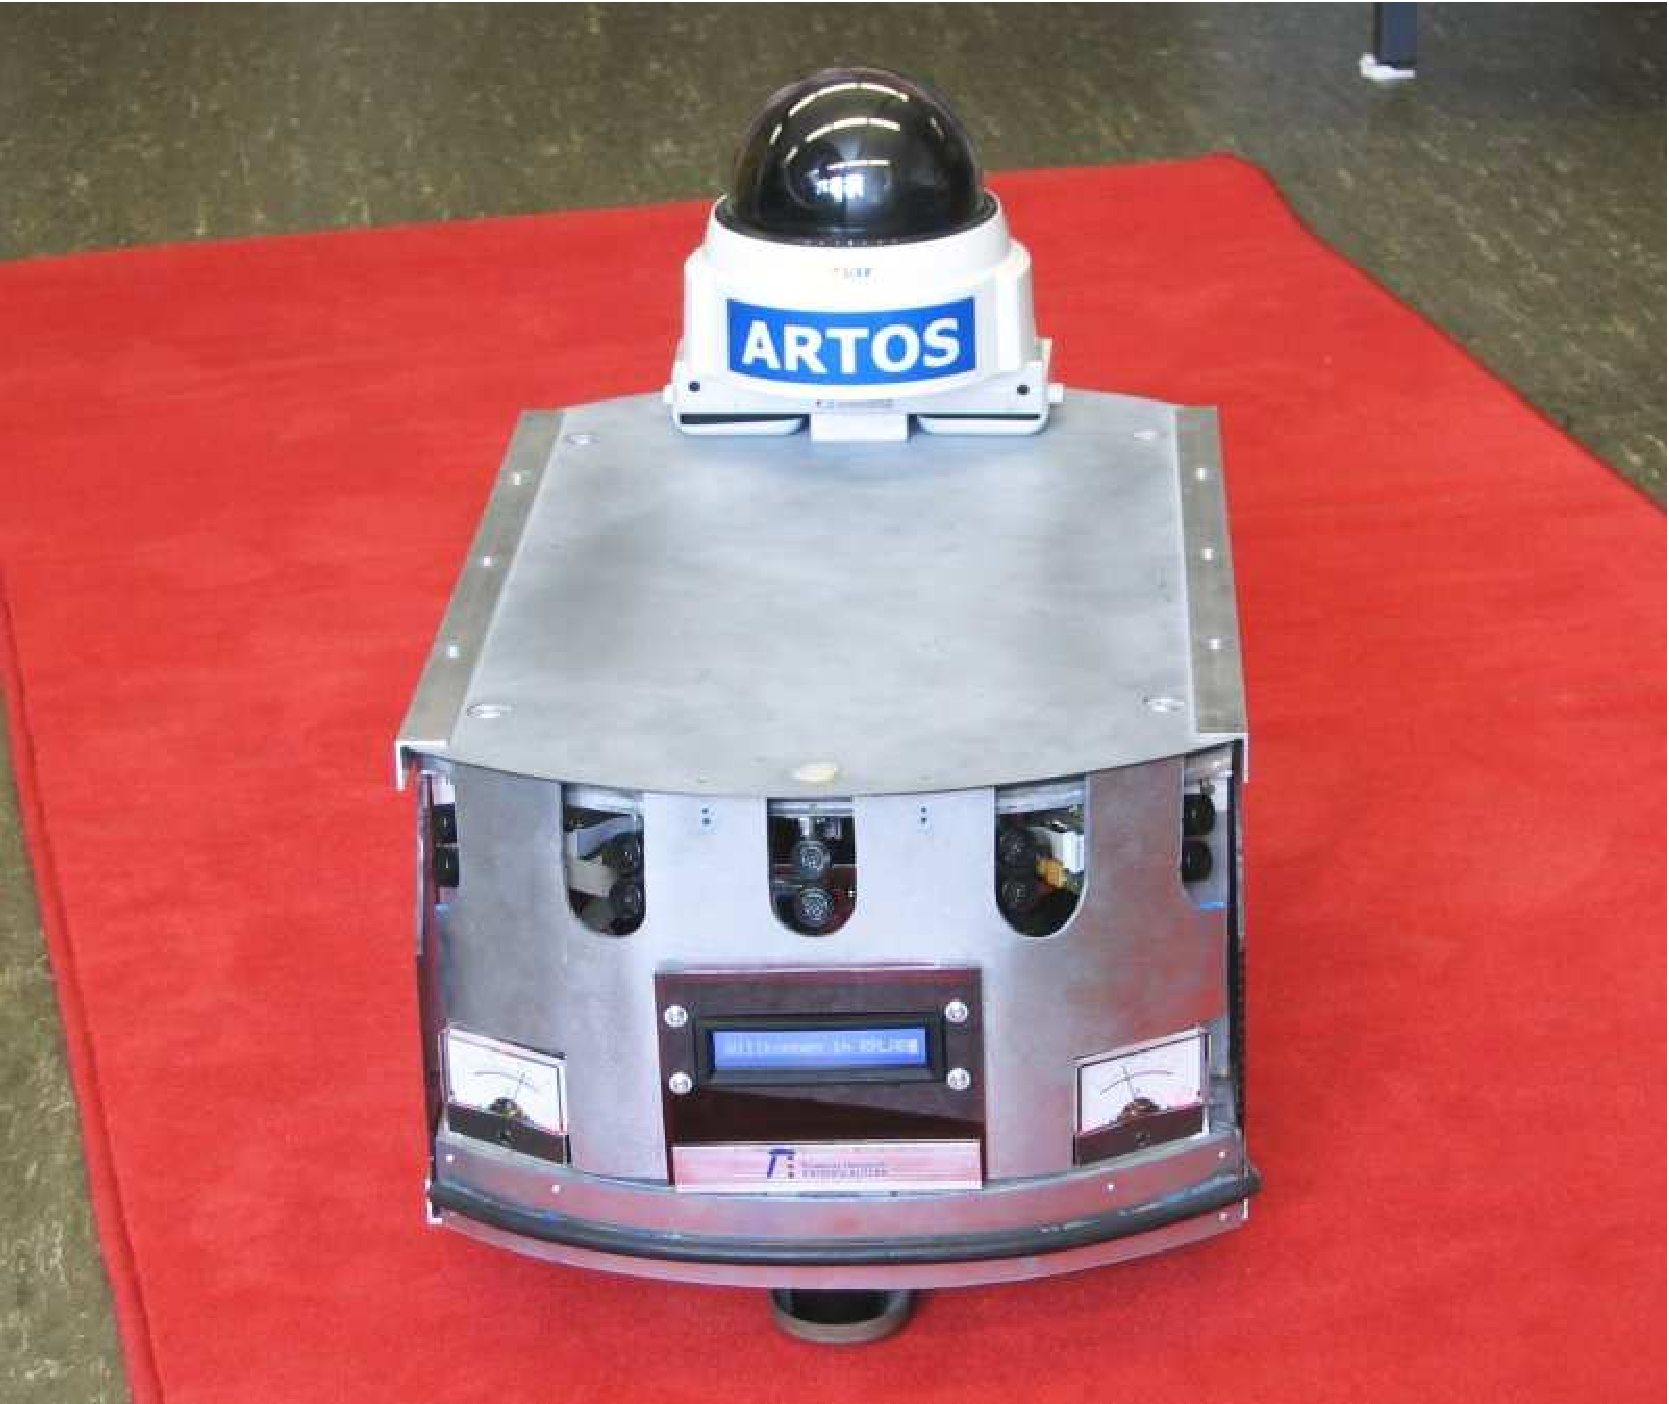
\includegraphics[height=5cm]{images/roter_teppich}
        \caption{Der mobile Roboter \RRLABartos (Autonomous Robot for Transport and Service).}
        \label{fig:ARTOS}
      \end{center}
    \end{minipage}
    \hspace{0.02\textwidth}
    \begin{minipage}{0.48\textwidth}
      \begin{center}
        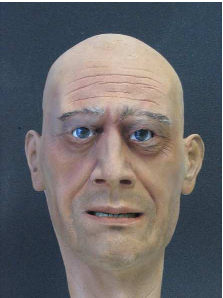
\includegraphics[height=5cm]{images/roman_mask}
        \caption{Der humanoide Roboter \RRLABroman (RObot huMAN interaction machine).}
        \label{fig:ROMAN}
      \end{center}
    \end{minipage}
  \end{center}
\end{figure}

The associated source code would look like this:

\begin{verbatim}
\begin{figure}
  \begin{center}
    \begin{minipage}{0.48\textwidth}
      \begin{center}
        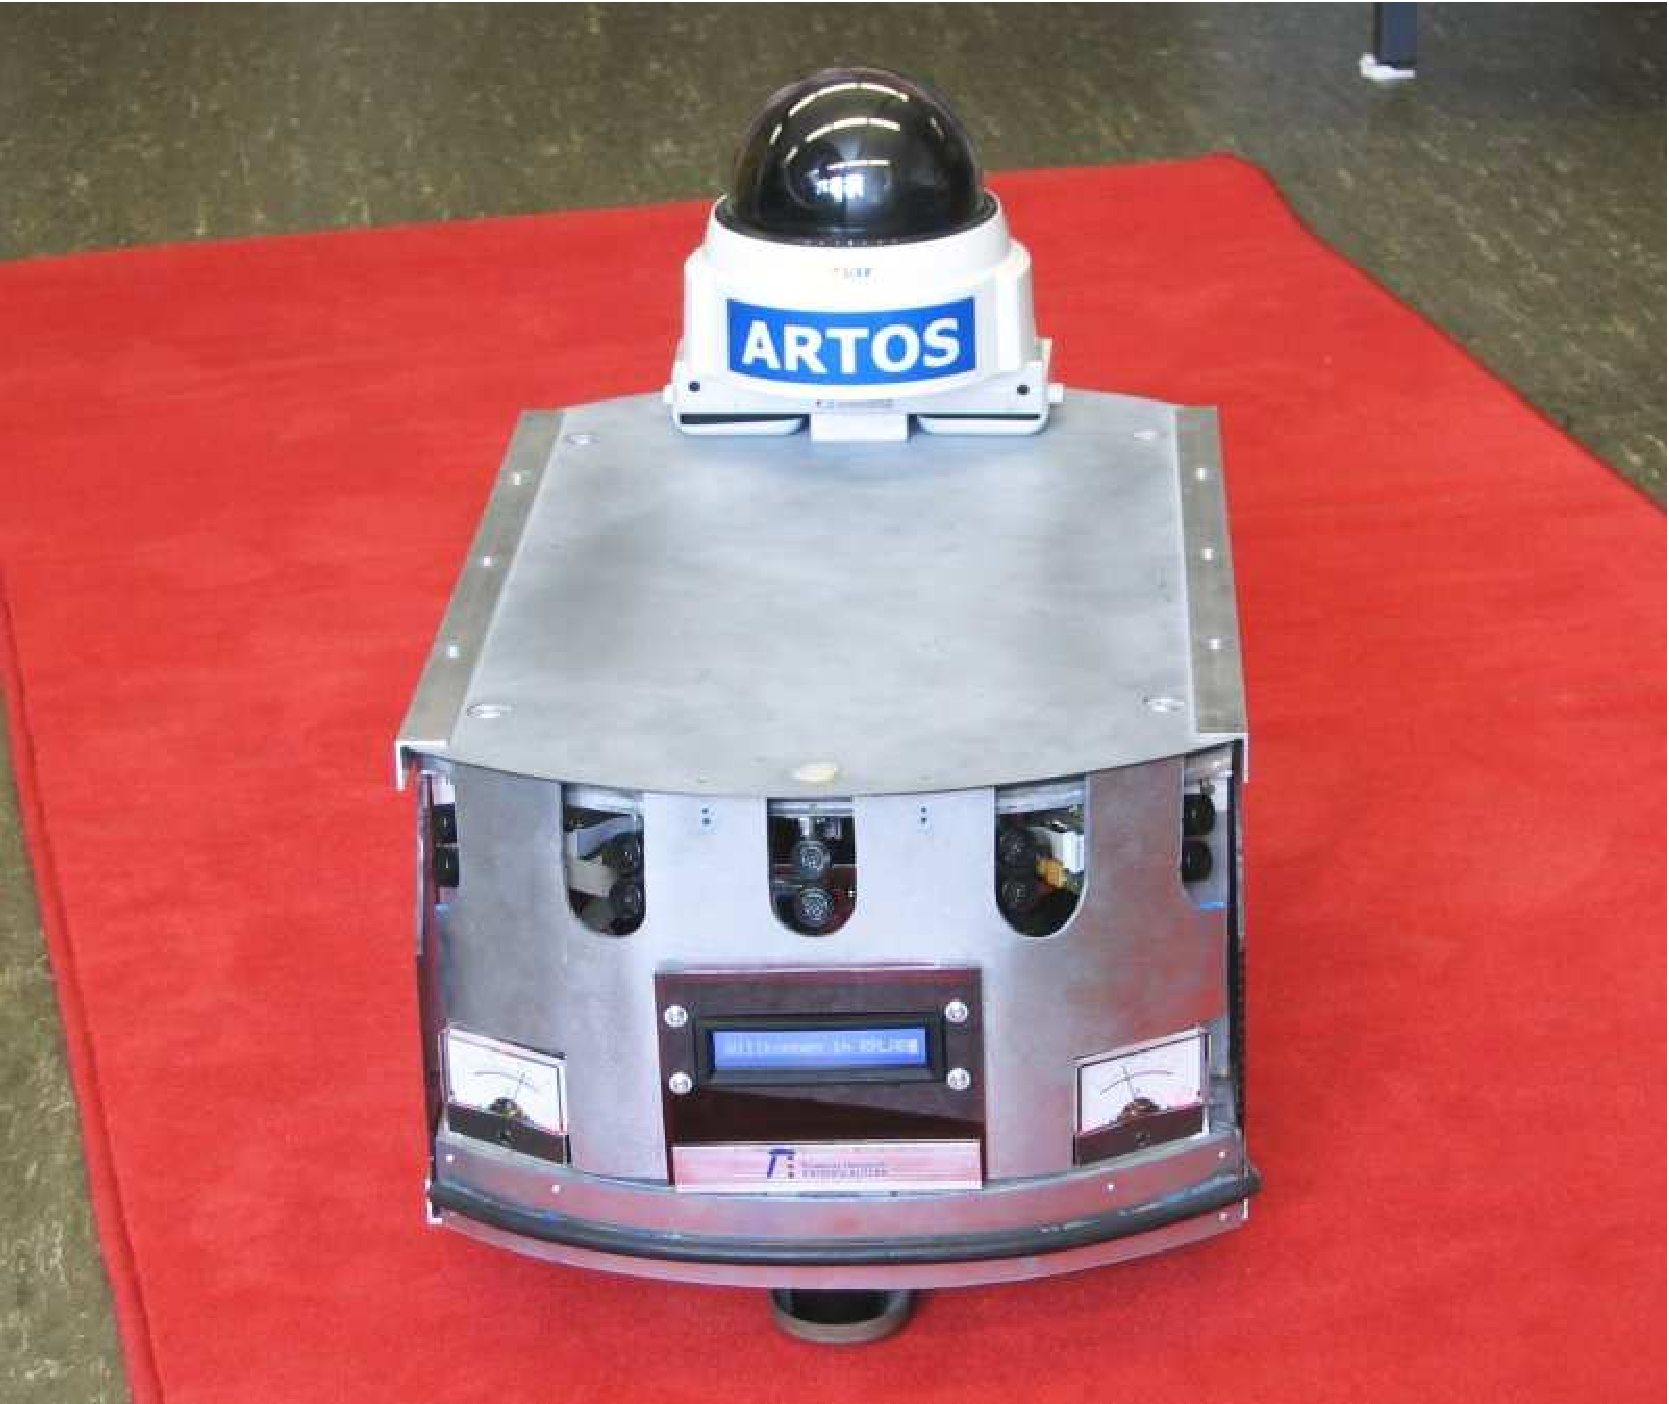
\includegraphics[height=5cm]{images/roter_teppich}
        \caption{Der mobile Roboter \RRLABartos 
            (Autonomous Robot for Transport and Service).}
        \label{fig:ARTOS}
      \end{center}
    \end{minipage}
    \hspace{0.02\textwidth}
    \begin{minipage}{0.48\textwidth}
      \begin{center}
        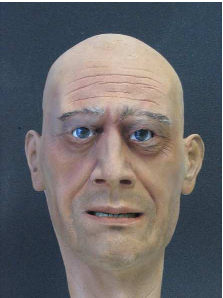
\includegraphics[height=5cm]{images/roman_mask}
        \caption{Der humanoide Roboter \RRLABroman 
            (RObot huMan interAction machiNe).}
        \label{fig:ROMAN}
      \end{center}
    \end{minipage}
  \end{center}
\end{figure}
\end{verbatim}


%%%%%%%%%%%%%%%%%%%%%%%%%%%%%%%%%%%%%%%%%%%%%%%%%%%%%%%%%%%%
\section{Tables}
\label{sec:floats:tables}
\index{Tables}The principles regarding the captioning of tables are similar to those for images. One can experiment with the number of lines, but the table appearance should remain consistent throughout the document. Table~\ref{tab:files} can serve as an example of tables.

%%%%%%%%%%%%%%%%%%%%%%%%%%%%%%%%%%%%%%%%%%%%%%%%%%%%%%%%%%%%
\section{Formulas und Units}
\label{sec:floats:formulas}
\index{Formulas} Formulas shouldn't get lost within the text, even if they're small (and unimaginative), such as $E=mc^2$, but rather be displayed in an \verb|equation| environment like so:
\begin{equation}
  \label{eq:einstein}
  E=mc^2 
\end{equation}
Generally, formulas should be numbered. For longer derivations, it suffices to label only important steps and the final result. When variables are mentioned in the text, such as the energy $E$ or the speed of light $c$ from Equation~\ref{eq:einstein}, these should be in math mode (e.g., \verb|$E$|). For complex formulas, the ,,amsmath'' package is included in the template. To display values with units, the ,,\verb|\unit|'' command is used, e.g., \unit[5]{mm} or \unitfrac[100]{km}{h} are generated using \verb|\unit[5]{mm}| or\ \verb|\unitfrac[100]{km}{h}|. If using the Euro symbol, include the ,,eurosym'' package.

%%%%%%%%%%%%%%%%%%%%%%%%%%%%%%%%%%%%%%%%%%%%%%%%%%%%%%%%%%%%
\section{Algorithms}
\label{sec:floats:algo}
\index{Algorithms} To visualize algorithms and special program sections, the functionality of the \verb|algorithm2e.sty| package can be employed. Both are supported, for instance, in \cite{WWWDante}, but generally aren't included in \LaTeX distributions, which is why we provide them.

\begin{algorithm}
  Create a 2D array\\
  Perform depth-first search:\\
\ForAll{nodes of tree U with coordinates $(x,y,z)$}{%
  \If{$z$-coordinate  of cell is greater than value in array at $(x,y)$}
    {Store $z$ at position  $(x,y)$ in 2D array}
}
Create Quadtree $G$\\
Perform depth-first search again:\\
\ForAll{nodes of tree $U$ with coordinates $(x,y,z)$}{%
  \If{coordinates match those stored in the 2D array}
    {Store $z$ for $(x,y)$ in Quadtree $G$}
}
\caption{Generating a global 2D map $G$ from an original map $U$}
\label{alg:example}
\end{algorithm}

The file \verb|algorithm2e.pdf| is attached as documentation. Generally, significant algorithms should be represented in pseudocode similar to Algorithm~\ref{alg:example} using these packages to enhance understanding. If it's necessary to include ,,actual'' source code (which mostly belongs in the appendix), the \LaTeX style \verb|listings.sty| is recommended, refer to Chapter~\ref{sec:floats:source_code}

Als Dokumentation ist die Datei  beigef\"ugt. Grunds\"atzlich
sollten wichtige Algorithmen als Pseudocode in der Art von
Algorithmus mithilfe dieser Pakete angegeben
werden, um das Verst\"andnis zu erleichtern. Sollte es tats\"achlich n\"otig
sein, ,,richtigen'' Quellcode einzuf\"ugen (der aber h\"ochstens mal in
den Anhang geh\"ort), ist der \LaTeX -Style \verb|listings.sty|
empfehlenswert, Kapitel~\ref{sec:floats:source_code}.


%%%%%%%%%%%%%%%%%%%%%%%%%%%%%%%%%%%%%%%%%%%%%%%%%%%%%%%%%%%%
\section{References}
\label{sec:floats:bib}
\index{References} All sources used must be listed in the bibliography, and references to them should be made at the corresponding text location. This is done with \verb|\cite{<label>}|, where \verb|<label>| corresponds to the entry in the BibTeX file. The name of the BibTeX file is passed to the \verb|literatur| macro in the main document (also refer to Chapter~\ref{sec:class:main}). For guidance on constructing the BibTeX file, take a look at \verb|literatur.bib| or consult appropriate literature (\cite{Lamport95}, \cite{WWWBibTex}). Additionally, examples for most possible BibTeX entries and explanations can be found in the file \verb|examples.bib|. Below are examples of the most important types:

\begin{itemize}
 \item Article in a journal~\cite{Albiez03}
 \item Book~\cite{Arkin98}
 \item Thesis~\cite{Luksch02}
 \item Dissertation~\cite{Breazeal00}
 \item Chapter in a Book~\cite{Mendel70}
 \item Chapter in a Collection~\cite{Ilg99}
 \item Conference proceedings~\cite{Berns07}
 \item Conference paper~\cite{Berns06}
 \item Technical report~\cite{Schaefer03}
\end{itemize}

The BibTeX layout generates references consisting of the last name of the first author and the last two digits of the publication year. When referencing URLs, the \verb|@Misc| entry can be used as demonstrated in \verb|literatur.bib|. As internet pages are subject to dynamic changes, they are not suitable for citing and referencing like books. Therefore, footnotes are a popular alternative for referencing internet pages.\footnote{http://rrlib.cs.uni-kl.de/}.


%%%%%%%%%%%%%%%%%%%%%%%%%%%%%%%%%%%%%%%%%%%%%%%%%%%%%%%%%%%%
\section{Index}
\label{sec:floats:index}
\index{Index} In larger works, creating an index can be useful. It's advisable to plan this from the start, making it easy to add index references at interesting points. This is done using \verb|\index{<keyword>}|, listing the <keyword> in the index directory along with the page number where the index command is located. Subpoints can be created with \verb|\index{<keyword>!<subpoint>}|. The index itself can be generated in the main document using the following macro: \verb|\RRLABindex|.

%%%%%%%%%%%%%%%%%%%%%%%%%%%%%%%%%%%%%%%%%%%%%%%%%%%%%%%%%%%%
\section{Additional Notes}
\index{Punctuation}
\index{Enumerations}

The ,,\verb|\itemize|'' environment is used for creating lists. Further instructions on punctuation are explained below:

\begin{itemize}
 \item If there isn't a complete sentence, start with lowercase after the bullet point.
 \item If a complete sentence follows a colon, start with a capital letter.
 \item No spaces are added before~.~,~!~?~:~;~,~etc.
 \item Quotation marks in German look like ,, (generated as \verb|,,|) while in English they appear  as `` (generated as \verb|``|).
 \item The closing quotation marks in both German and English look like '' (generated as \verb|''|).
 \item  There are four types of dashes: - (generated as \verb|-|), -- (generated as \verb|--|), --- (generated as \verb|---|) and $-$ (generated as \verb|$-$|). 

 The first is used as a hyphen, en dash, or em dash. In German, words consisting of several nouns are written together or alternatively separated by hyphens. In English, hyphens are omitted. For example:
 Mensch"=Roboter"=Interaktion bzw.\ human-robot interaction in English. Additionally, words composed of both English and German words are hyphenated. 

 The second dash is used as an em dash in German and for ranges and compound words.

 The third is used as an em dash in English and for tables. In German, spaces are added before and after the dash; in English, they are not (,,Du magst ja recht haben -- aber ich sehe das ganz anders.'' "the fire drill---it was chaos'').


 The last dash is the minus sign.
 
 \item Regarding number representation, there are several methods: traditionally, numbers from 0--11 are written as words, but newer conventions allow all numbers to be written as digits. Whichever style is chosen, consistency is key. 
\end{itemize}

If using the German language package, a hyphen determines where a word can be split (only at that point). This can lead to problems with compound words (e.g., Mensch"=Roboter"=Interaktion). To avoid this issue, hyphens can be coded as follows: \verb|Mensch"=Roboter"=Interaktion|. When referencing a webpage, it's best to do so with a footnote\footnote{\url{http://agrosy.informatik.uni-kl.de/}}. The code looks like: \verb|\footnote{\url{http://agrosy.informatik.uni-kl.de/}}|.


%%%%%%%%%%%%%%%%%%%%%%%%%%%%%%%%%%%%%%%%%%%%%%%%%%%%%%%%%%%%
\section{Darstellen von Quellcode-Fragmenten}
\label{sec:floats:source_code}
\index{Quellcode}

For C++ code, the following can be used:

\begin{verbatim}
\lstloadlanguages{C++}
\lstset{language=[GNU]C++, basicstyle=\tiny, breakautoindent,
breaklines, deletekeywords={LOCAL_DEBUG, MODULE_DEBUG, \#undef},
keywordstyle=\textbf, commentstyle=\color{Gray}, alsoletter=
{\#, \"}, emph={bool, byte, short, int, long, float, double, 
long double, char, const, static}, emphstyle=\color{red}, 
stringstyle=\color{red}, morecomment=[l][\color{green}]{\#}, 
numberstyle=\color{blue}, morecomment=[s][\color{blue}]
{/*}{*/}} 
\begin{lstlisting} 
  .
  .
  .
\end{verbatim}

This will render it relatively similar to how it appears in kdevelop.

\lstloadlanguages{C++}
\lstset{language=[GNU]C++, basicstyle=\tiny, breakautoindent, breaklines, deletekeywords={LOCAL_DEBUG, MODULE_DEBUG, \#undef},keywordstyle=\textbf, commentstyle=\color{Gray}, alsoletter={\#, \"}, emph={bool, byte, short, int, long, float, double, long double, char, const, static}, emphstyle=\color{red}, stringstyle=\color{red}, morecomment=[l][\color{green}]{\#}, numberstyle=\color{blue}, morecomment=[s][\color{blue}]{/*}{*/}}

\begin{lstlisting} 
// this is a -*- C++ -*- file
//----------------------------------------------------------------------
/*!\file    mbbDrive.C
 *
 * \author   Jochen Hirth
 * \date    18.04.06
 *
 * $Revision: 1.3 $
 * $Id: NullBehaviourBasedModule.C,v 1.3 2005/10/04 11:17:39 martin Exp $
 *
 */ 
//----------------------------------------------------------------------
// Includes
//----------------------------------------------------------------------

#include "mbbDrive.h"

//----------------------------------------------------------------------
// Module Debug
//----------------------------------------------------------------------
//#undef MODULE_DEBUG
#define MODULE_DEBUG
#include "kernel/ModuleDebug.h"

//----------------------------------------------------------------------
// Debugging
//----------------------------------------------------------------------
#undef LOCAL_DEBUG 
//#define LOCAL_DEBUG
#include "kernel/LocalDebug.h"

//----------------------------------------------------------------------
// defines and consts
//----------------------------------------------------------------------

//----------------------------------------------------------------------
// class mbbDrive constructor
//----------------------------------------------------------------------
mbbDrive::mbbDrive( tParent *parent, tDescription name, tBehBBHandler* _beh_bb_handler, bool fixit )
        : tBehaviourBasedModule( parent, name,
                                 eSI_DIMENSION, eSO_DIMENSION, eCI_DIMENSION, eCO_DIMENSION,
                                 si_description, so_description, ci_description, co_description, _beh_bb_handler )
{

    sigmoid = new tSigmoid( tSigmoid::eSIG_RISE, 0., 1. );
}

//----------------------------------------------------------------------
// class mbbDrive destructor
//----------------------------------------------------------------------
mbbDrive::~mbbDrive()
{
    delete sigmoid;
}

\end{lstlisting}

However, you can also load the code or selected lines from a file and display line numbers:

\begin{verbatim}
\lstinputlisting[numbers=left,linerange={1-4,7-26}]{mbbDrive.cpp}
\lstinputlisting[numbers=left,linerange={33-43}]{mbbDrive.cpp}
\end{verbatim}

Und das sieht dann so aus:

\lstinputlisting[numbers=left,linerange={1-4,7-26}]{mbbDrive.cpp}
\lstinputlisting[numbers=left,linerange={33-43}]{mbbDrive.cpp}

For \textsc{xml}-code, the following setting is appropriate:

\begin{verbatim}
\lstset{language=xml, basicstyle=\tiny, breakautoindent,
 breaklines,keywordstyle=\textbf, keywordsprefix=<, 
identifierstyle=\color{green}, stringstyle=\color{red}} 
\begin{lstlisting} 
  .
  .
  . 
\end{verbatim}

The output will look like this:

\lstset{language=xml, basicstyle=\tiny, breakautoindent, breaklines, keywordstyle=\textbf, keywordsprefix=<, identifierstyle=\color{green}, stringstyle=\color{red}}

\begin{lstlisting} 
<?xml version="1.0" encoding="ISO-8859-1"?>
<data xmlns:xsi="http://www.w3.org/2001/XMLSchema-instance"
 xsi:schemaLocation="Belami DoAmi_dialog_description_scheme(v1.2).xsd"
 xmlns:belami="http://www.w3.org/2001/Belami"
 xmlns="http://www.w3.org/2001/Belami">
    <platform type="desktop">
        <SUI_settings>
            <tts_settings context="free" voice="0" speed="100" activate="immediately"/>
            <asr_settings activate="immediately" timeout="4" acknowledge="true"/>
        </SUI_settings>	       
	<dialog dialog_id="Welcome">
		<SUI_dialog>
	    	<SUI_settings>
                </SUI_settings>
			<prompt>Hallo! Ich bin Roman, der humanoide Roboterkopf der technischen Universiteet Kaiserslautern. Meine Aufgabe ist es, mit Menschen zu kommunizieren. Hierzu kann ich emotionale Gesichtsausdruicke einsetzen.</prompt>
			<goto mark="Recognize"/>
	</SUI_dialog>
        </dialog>

\end{lstlisting}

Additionally, the "listings" package offers the ability to display many other programming languages. For more information, please refer to the accompanying documentation.

%%% Local Variables: 
%%% mode: latex
%%% TeX-master: "howto"
%%% End: 
